\newpage
\section{Aplikacja}
\label{sec:app}
Aplikacja stanowi praktyczne wykorzystanie rozwiązań badanych w ramach części badawczej. Jest ona demem technologicznym, którego celem jest demonstracja praktycznego zastosowania badanych modeli oraz przedstawienia możliwości wykorzystania uczenia maszynowego w aplikacji mobilnej. 
\subsection{Technologie}
Aplikacja została zaimplementowana w języku Dart z wykorzystaniem środowiska Flutter. Do testowania aplikacji wykorzystano emulator dostępny w środowisku Android Studio symulujący telefon mobilny z systemem Android.. Do implementacji modelu wykorzystano bibliotekę TensorFlow. Zarówno TensorFlow, jak i Flutter są produktami od firmy Google, dzięki czemu są ze sobą kompatybilne i umożliwiają użycie modelu bezpośrednio na urządzeniu mobilnym, dzięki czemu aplikacja może wykonywać klasyfikację bez dostępu do sieci internetowej. Do konwersji modelu zapisanego w formacie \textit{.pth} do formatu \textit{.tf} wykorzystywanego przez TensorFlow został wykorzystany ekosystem wymiany modeli Onnx.


\subsection{Implementacja modelu}
 W aplikacji wykorzystano model MobileNetV3Small. Model ten został zaprojektowany z myślą o zastosowaniach na urządzeniach mobilnych. Dodatkowo, na podstawie przeprowadzonych badań, udało się stwierdzić, że modele z tej rodziny stanowią dobry kompromis między skutecznością a wymaganiami sprzętowymi.

Model został przekonwertowany z wcześniej zapisanych wag w formacie \textit{.pth} używanym przez bibliotekę PyTorch na format \textit{.tf} używany przez TensorFlow. Do tego został użyty ekosystem Onnx. Dzięki temu model może być umieszczony bezpośrednio w plikach aplikacji, a sama klasyfikacja wykonywana lokalnie, bez potrzeby dostępu do serwera. 

\subsection{Widoki i działanie}

\begin{figure}[H]
	\centering
	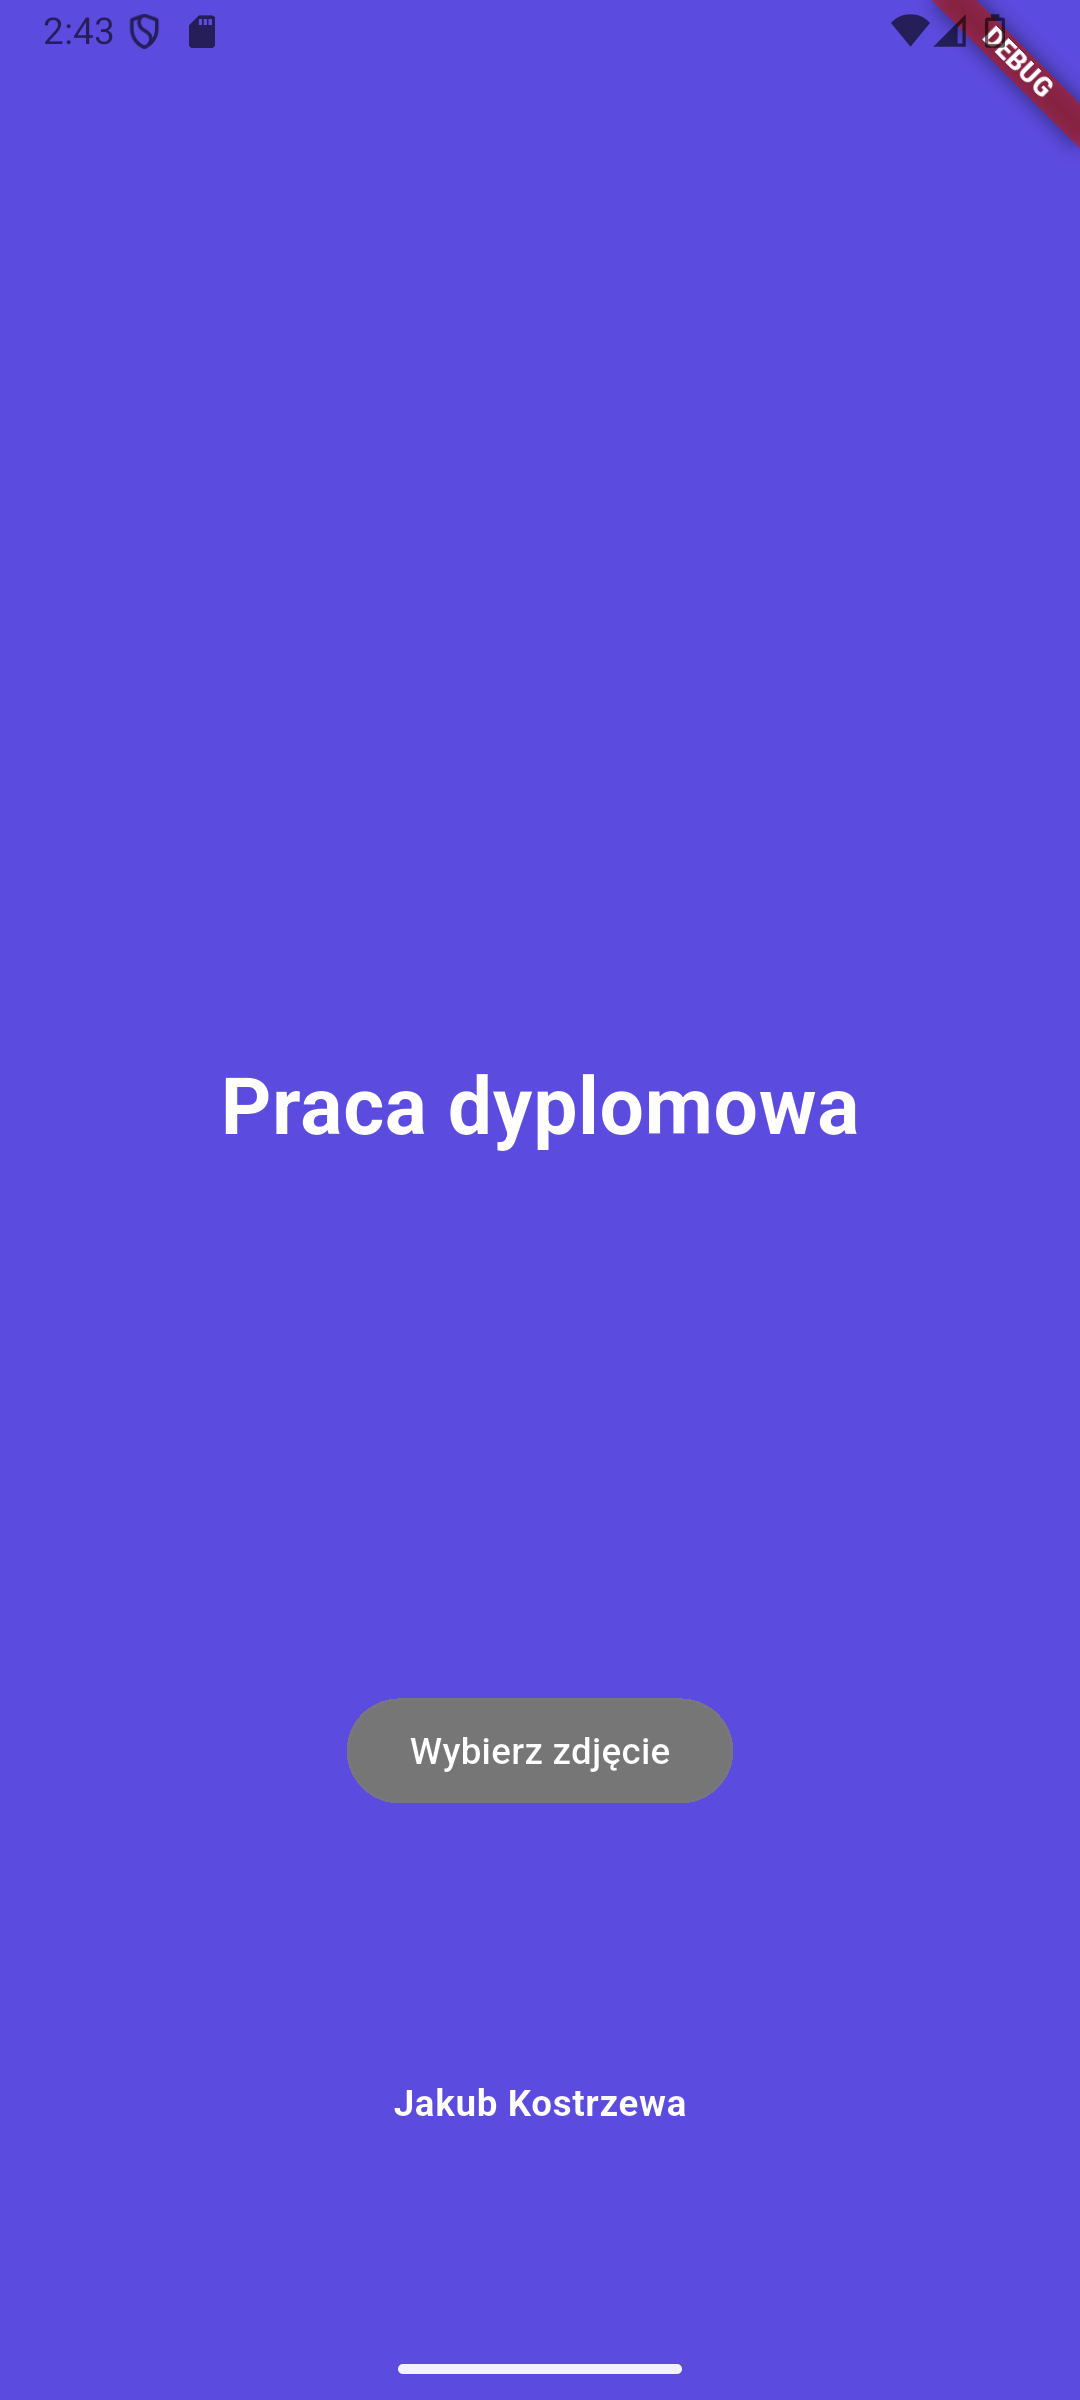
\includegraphics[width=0.3\textwidth]{img/aplikacja-1.png}
	\hspace{0.05\textwidth}
	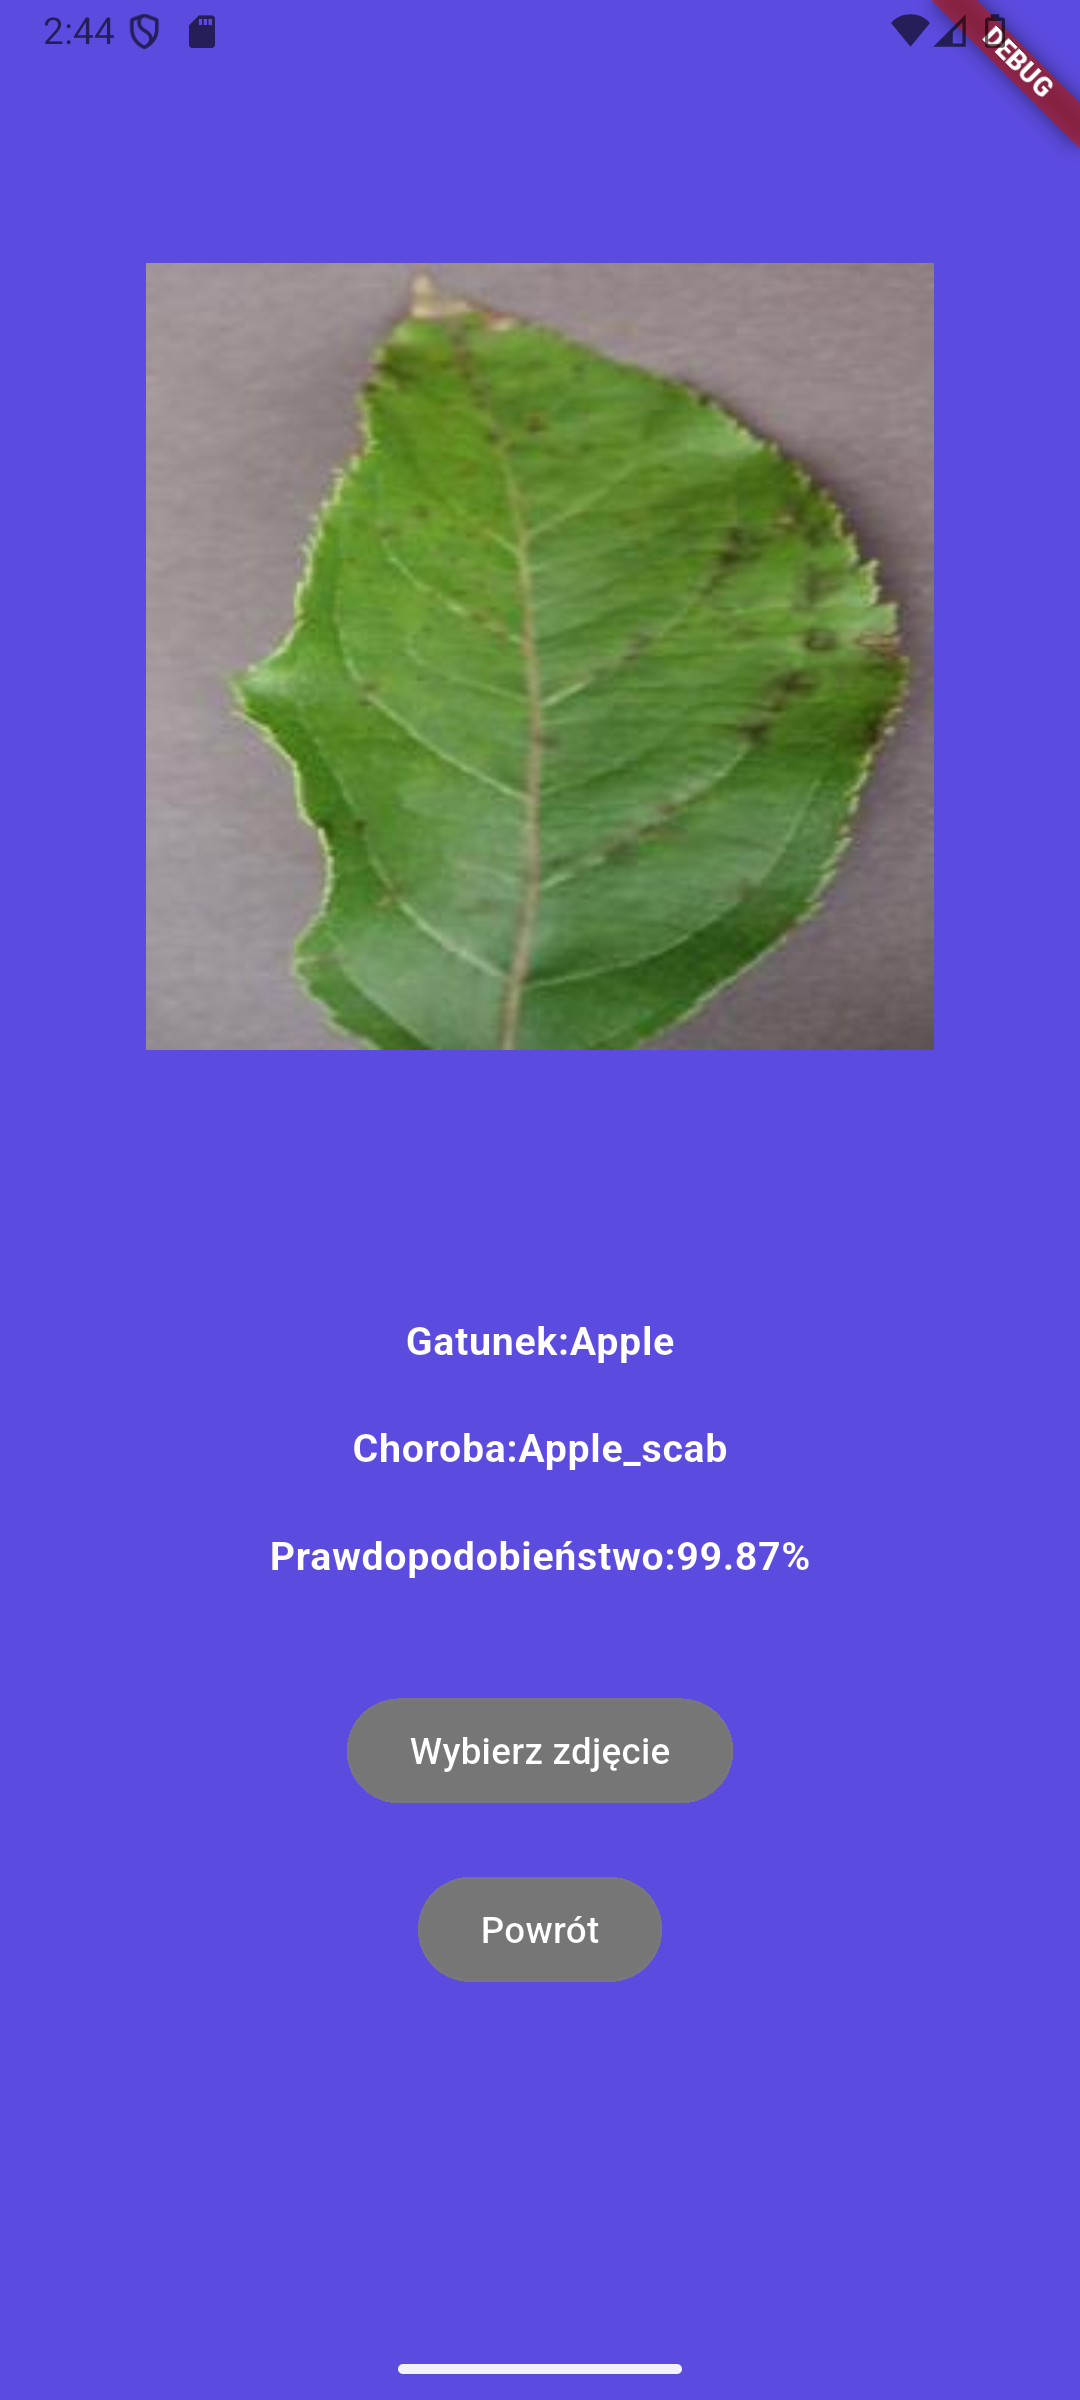
\includegraphics[width=0.3\textwidth]{img/aplikacja-2.png}
	\caption{Zdjęcie ekranu startowego oraz ekranu z wynikami }
	\label{fig:menu}
\end{figure}

W ramach pierwszego widoku aplikacja pozwala użytkownikowi na kliknięcie przycisku \textit{Wybierz zdjęcie}. Spowoduje to otwarcie galerii, gdzie użytkownik może wybrać zdjęcie przeznaczone do klasyfikacji.


W ramach widoku drugiego aplikacja wyświetla wyniki klasyfikacji uzyskane przez model oraz wybrane wcześniej zdjęcie. Użytkownik otrzymuje informację o gatunku rośliny, rozpoznanej chorobie oraz wartości prawdopodobieństwa poprawnie wykonanej klasyfikacji.

 Na tym ekranie znajdują się też dwa przyciski - \textit{Wybierz zdjęcie} oraz \textit{Powrót}. Kliknięcie pierwszego przycisku spowoduje ponowny wybór zdjęcia oraz ponowne wyświetlenie, już nowych, wyników. Drugi przycisk pozwala na powrót do ekranu startowego aplikacji.



